\section{Product Matching}\label{sec:sec_product_matching}

The product matching module is responsible for identifying and linking identical products across different websites.
This is done in order to provide users with a view of the same product available on different websites, along with their respective prices and other relevant information.
This task can be considered to be a document matching problem, where the goal is to determine whether two given product pages refer to the same product or not.
The literature suggests that most document matching techniques rely on two phases: a candidate generation (filtering) phase and a candidate ranking (verification) phase.
The candidate generation phase is a relatively computationally inexpensive process that aims to reduce the number of candidate pairs to be compared in the subsequent candidate ranking phase, which is a more computationally expensive process that aims to accurately determine whether the candidate pairs refer to the same product or not.
Figure~\ref{fig:product_matching} illustrates how filtering and verification phases are used in the product matching module to identify and link identical products across different websites.

\begin{figure}[h]
    \centering
    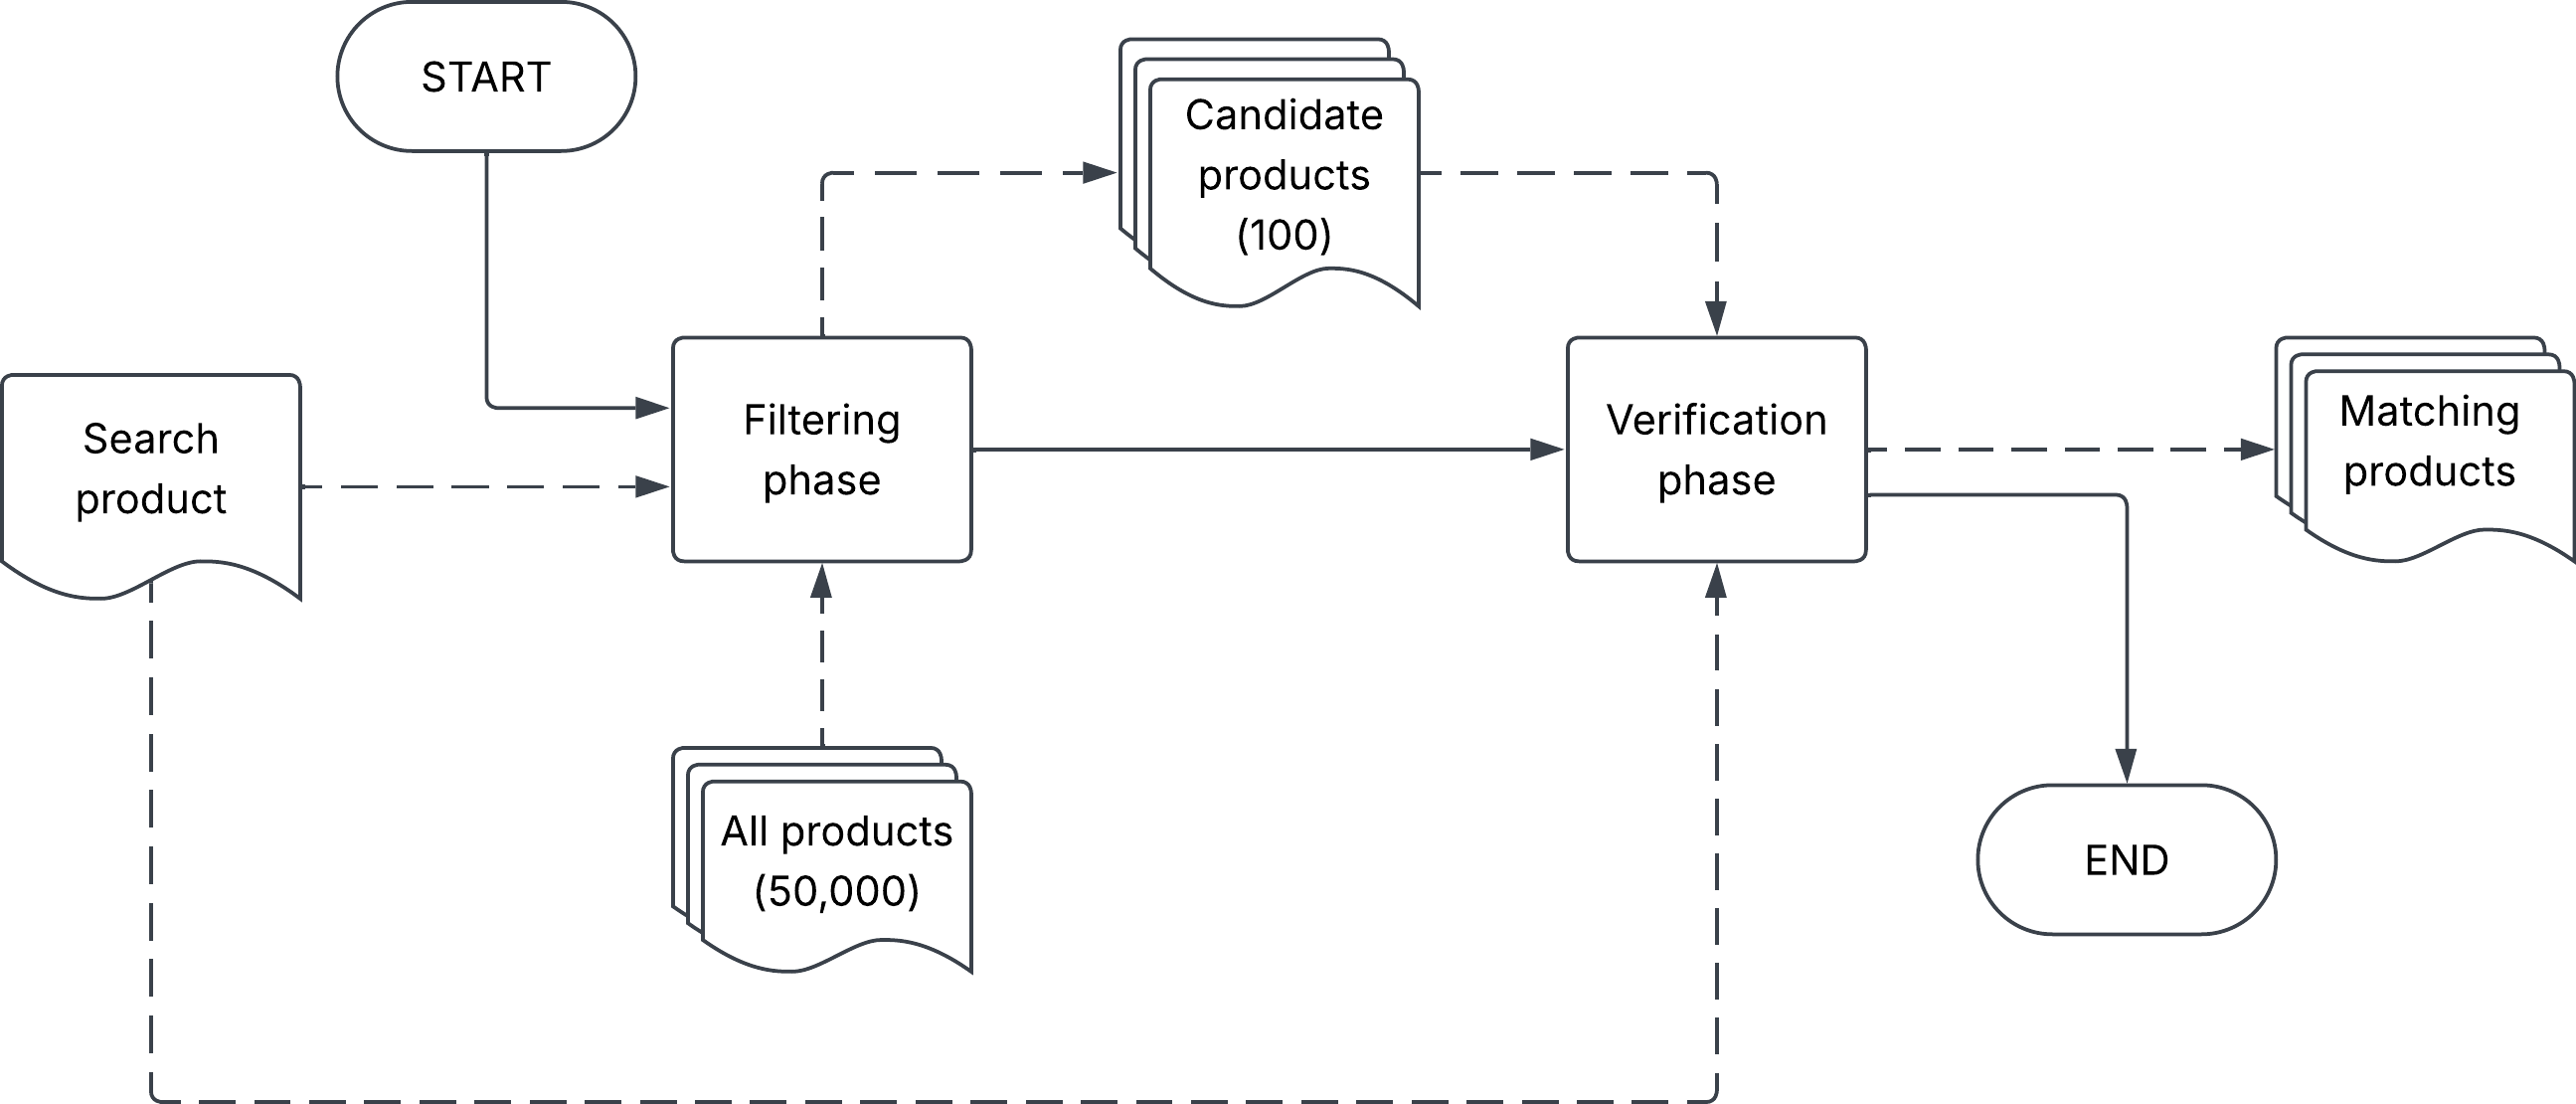
\includegraphics[width=1\textwidth]{images/filtering_and_verification_phases}
    \caption{Overview of the product matching module.}
    \label{fig:product_matching}
\end{figure}

\subsection{Comparison of Different Approaches}\label{subsec:sec_product_matching_comparison_of_approaches}
Before deciding on the approaches to be used for the candidate generation and candidate ranking phases, a comparison of different approaches was conducted.
\begin{enumerate}
    \item \textbf{Trigram similarity with title only:} This approach involves computing the trigram Jaccard similarity between the titles of the two product pages.
    \item \textbf{Edit distance with title only:} This approach involves computing the edit distance between the titles of the two product pages.
    \item \textbf{BM-25 algorithm:} This approach involves using the BM-25 algorithm to compute the similarity between the two product pages based on their titles and descriptions.
    \item \textbf{RexBERT embeddings on title only (256 dimensions):} This approach involves using a pre-trained RexBERT model to generate embeddings for the titles of the two product pages, and then computing the cosine similarity between the embeddings.
    RexBERT is a transformer-based model that is pre-trained on a large corpus of e-commerce product data, and is able to capture the semantic information in products.
    \item \textbf{RexBERT embeddings on body (256 dimensions):} This approach involves using a pre-trained RexBERT model to generate embeddings for the bodies of the two product pages, and then computing the cosine similarity between the embeddings.
    This was chosen to investigate whether a model pre-trained on a large corpus of e-commerce product data could provide better performance other vector embedding models.
    \item \textbf{RexBERT embeddings on body (768 dimensions):} This approach involves using a pre-trained RexBERT model to generate embeddings for the bodies of the two product pages, and then computing the cosine similarity between the embeddings.
    \item \textbf{RexBERT embeddings on body (1024 dimensions):} This approach involves using a pre-trained RexBERT model to generate embeddings for the bodies of the two product pages, and then computing the cosine similarity between the embeddings.
    \item \textbf{RexBERT embeddings on body converted to Markdown (768 dimensions):} This approach involves converting the bodies of the two product pages to Markdown format, generating embeddings using a pre-trained RexBERT model, and then computing the cosine similarity between the embeddings.
    This was chosen to investigate whether converting the bodies of the product pages to Markdown format could provide information in a more friendly format that could improve the performance of the product matching module.
    \item \textbf{MarkupLM embeddings on body (768 dimensions):} This approach involves using a pre-trained MarkupLM model to generate embeddings for the bodies of the two product pages, and then computing the cosine similarity between the embeddings.
    This was chosen to investigate whether the HTML structure of the product pages could provide additional information that could improve the performance of the product matching module.
\end{enumerate}

For all the vector-based approaches above, the cosine similarity was used as the similarity measure.
The results of each of the above approaches are summarized in Table~\ref{tab:product_matching_approaches}, which shows the compute required for generating and comparing the embeddings, the similarity scores for matching and non-matching products, the difference between the two similarity scores, and the performance difference between the two similarity scores.

\begin{table}[h]
    \centering
    \small
    \renewcommand{\arraystretch}{1.4}
    \begin{tabularx}{\textwidth}{p{3.5cm} p{1.4cm} p{1.4cm} p{1.9cm} p{1.9cm} p{1.5cm} p{1.5cm}}
        \toprule
        \textbf{Technique} & \textbf{Compute for Generation} & \textbf{Compute for Comparison} & \textbf{Matching Products} & \textbf{Non-Matching Products} & \textbf{Difference} & \textbf{Percentage Difference} \\
        \midrule
        Trigram similarity with title only & N/A & VERY LOW & 0.73 & 0.52 & 0.21 & 38.33\% \\
        \midrule
        Edit distance with title only & N/A & VERY LOW & 0.66 & 0.57 & 0.09 & 16.57\% \\
        \midrule
        BM-25 algorithm & MEDIUM & LOW & 0.58 & 0.10 & 0.48 & 473.69\% \\
        \midrule
        RexBERT embeddings on title only (256 dimensions) & LOW & LOW & 0.96 & 0.93 & 0.02 & 1.78\% \\
        \midrule
        RexBERT embeddings on body (256 dimensions) & MEDIUM & MEDIUM & 0.98 & 0.97 & 0.01 & 1.03\% \\
        \midrule
        RexBERT embeddings on body (768 dimensions) & HIGH & MEDIUM & 0.92 & 0.86 & 0.06 & 6.98\% \\
        \midrule
        RexBERT embeddings on body (1024 dimensions) & HIGH & HIGH & 0.93 & 0.93 & 0.00 & 0.00\% \\
        \midrule
        RexBERT embeddings on body converted to markdown (768 dimensions) & HIGH & MEDIUM & 0.91 & 0.88 & 0.03 & 3.41\% \\
        \midrule
        MarkupLM embeddings on body (768 dimensions) & VERY HIGH & MEDIUM & 0.97 & 0.93 & 0.04 & 4.30\% \\
        \bottomrule
    \end{tabularx}
    \caption{Comparison of different product matching approaches}
    \label{tab:product_matching_approaches}
\end{table}

Based on these results, several observations were made:
\begin{itemize}
    \item The trigram similarity approach was found to be a good candidate for the candidate generation phase, as it was able to achieve a relatively high similarity score for matching products while being computationally inexpensive to compute.
    \item The BM-25 algorithm at first seemed to be ideal for the candidate ranking phase as it showed a very high difference between the similarity scores for matching and non-matching products, but it was found that this technique aggressively focussed on precision at the cost of recall, which is not ideal for the candidate ranking phase.
    \item The RexBERT embeddings on body (768 dimensions), while not the best performing approach overall, showed the most promise out of the vector embedding approaches.
\end{itemize}

None of the embedding models showed great performance as these models were not pre-trained on web-based corpora.
Even for models like RexBERT, which are pre-trained on e-commerce data, distinguishing between matching and non-matching product pairs was difficult because the overall variety of e-commerce products is very large.
The same product model with slightly different variations (e.g. colour, storage, memory), or even two different models, but very similar characteristics (e.g.\ high-end flagship smartphones) would appear very close together in the vector space.
Furthermore, the models were more likely to place products from the same site close together due to the common features/patterns that are available in the pages themselves and how they choose to organize information.

\subsection{Candidate Generation (Filtering) Phase}\label{subsec:sec_product_matching_filtering_phase}
During this phase, when given a product, the goal is to generate a relatively small number of candidate pairs that are likely to refer to the same product.
There are two main criteria to be considered when designing the candidate generation phase:
\begin{itemize}
    \item High recall: The candidate generation phase should aim to generate as many true positive pairs as possible, even if it means generating some false positive pairs.
    This is because the subsequent candidate ranking phase will be responsible for filtering out the false positives.
    \item Low computational cost: The candidate generation phase should be computationally inexpensive, as it will be applied to a large number of products and candidate pairs.
\end{itemize}

Considering the types of data available at this point, the technique opted for was to use the names of the products to generate candidate pairs.
For a given product, another page was considered to be a matching candidate if the trigram Jaccard similarity between the two product names was greater than a certain threshold.
This specific metric was chosen because it is relatively computationally inexpensive to compute, and it is able to capture the similarity between two strings even if they have minor differences in spelling or formatting.
Moreover, there is built-in support for computing trigram similarity in PostgreSQL via the \texttt{pg\_trgm} extension, which allows efficient computation of the similarity between two strings.
This also had the added benefit of allowing the candidate generation phase to be implemented as a SQL query, which is relatively easy to implement and maintain, without the need for additional infrastructure or services which helped in keeping the system simple and cost-effective.

Trigram Jaccard similarity is a measure of similarity between two strings, which is defined as the size of the intersection of the sets of trigrams (three-character sequences) in the two strings divided by the size of the union of the sets of trigrams in the two strings.
An example of this is illustrated in Figure~\ref{fig:trigram_jaccard_similarity}.

\begin{figure}
    \centering
    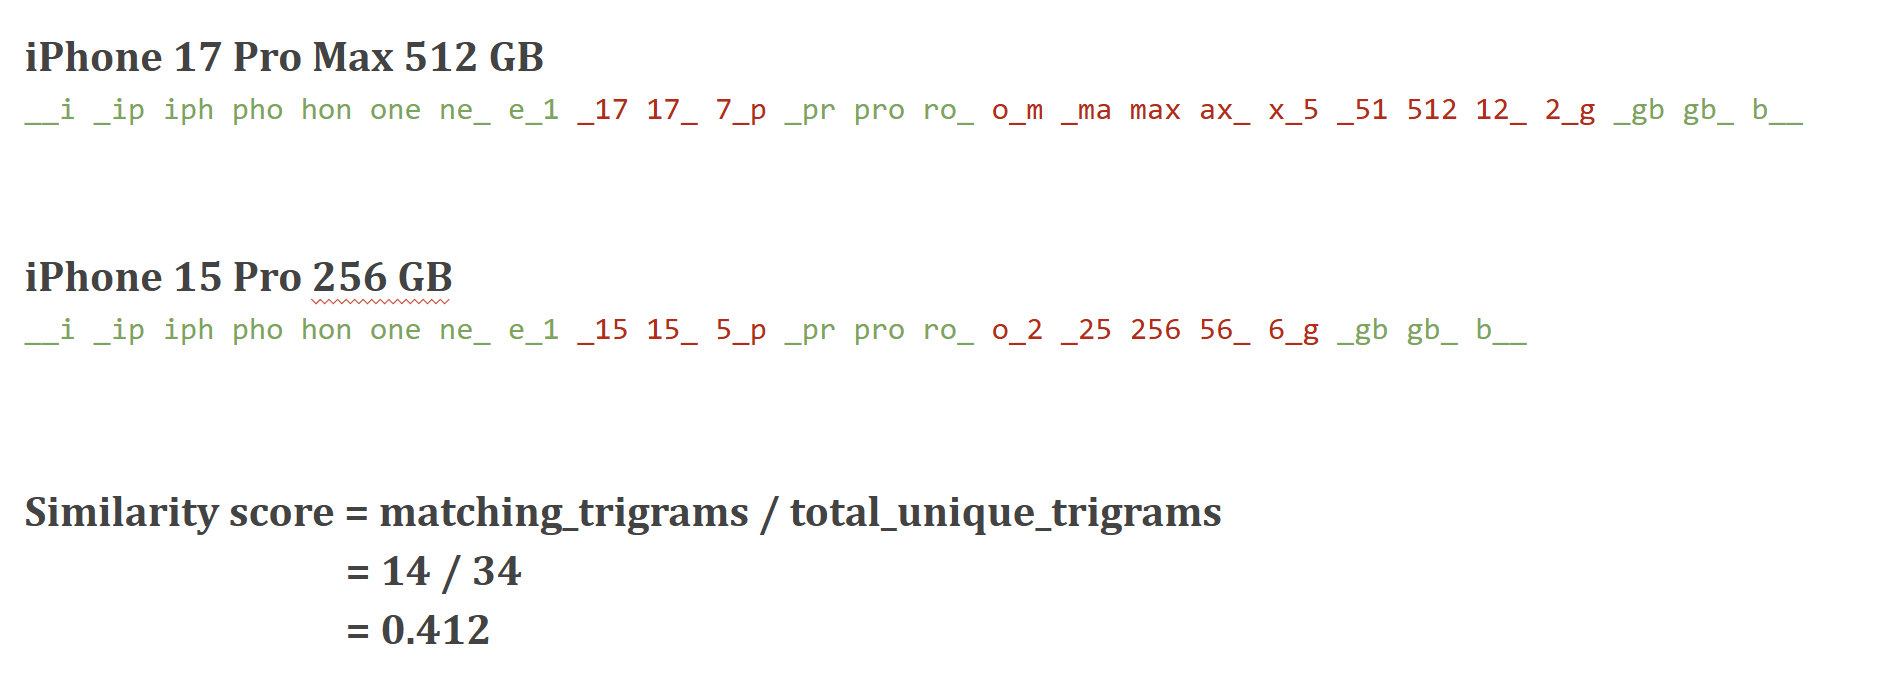
\includegraphics[width=1\textwidth]{images/trigram_similarity}
    \caption{Example of trigram Jaccard similarity between two product titles.}
    \label{fig:trigram_jaccard_similarity}
\end{figure}

In order to allow the maximum flexibility in terms of the threshold to be used for generating candidate pairs, the threshold was made configurable, but a default value of 0.3 was used, which was found to be a good balance between recall and computational cost.

\subsection{Candidate Ranking (Verification) Phase}\label{subsec:sec_product_matching_verification_phase}
During this phase, the goal is to accurately determine whether the candidate pairs generated in the previous phase refer to the same product or not.
This is a more computationally expensive process, as it involves comparing the candidate pairs using more sophisticated techniques, such as machine learning models or vector-based similarity measures.
For this phase, both precision and recall are important, as the goal is to accurately identify the true positive pairs while minimizing the number of false positives.

The literature suggested two main approaches for the candidate ranking phase: a machine learning approach and a vector-based approach.
A machine-learning based approach involves training a machine learning model to classify the candidate pairs as either matching or non-matching, based on a set of features extracted from the product pages.
This approach was considered to be infeasible as it would require the model to be online at all times, which would have been expensive.
Unlike the page classification and information extraction modules, it was also not possible to have pre-computed results for all product pairs as the number of pairs would be exponential in the number of products, which would have been infeasible to store and maintain.

Therefore, a vector-based approach was chosen, which involves representing the product pages as vectors in a high-dimensional space and computing the similarity between the vectors to determine whether the candidate pairs refer to the same product or not.
Vector similarity measures such as cosine similarity or Euclidean distance can be used to compute the similarity between the vectors, and a threshold can be set to determine whether the candidate pairs are considered to be matching or not.

This process can also be implemented in three phases.
\begin{enumerate}
    \item \textbf{Fine-tuning phase:} In this phase, a pre-trained language model is fine-tuned on a labelled dataset of positive and negative product pairs to learn a vector representation of the product pages that captures the semantic similarity between them.
    \item \textbf{Vector generation phase:} In this phase, the fine-tuned model is used to generate vector representations for all product pages in the database.
    \item \textbf{Matching phase:} In this phase, the vector representations of the candidate pairs are compared using a similarity measure, and a threshold is set to determine whether the candidate pairs are considered to be matching or not.
\end{enumerate}

\subsubsection{Fine-Tuning Phase}\label{subsubsec:sec_product_matching_fine_tuning_phase}

As shown in Table~\ref{tab:product_matching_approaches}, while the embedding models did not show great performance in distinguishing between matching and non-matching products, these models can be improved using contrastive fine-tuning, which is a technique that involves training the model to minimize the distance between the embeddings of matching product pairs while maximizing the distance between the embeddings of non-matching product pairs.
This is done by providing the model with:
\begin{itemize}
    \item \textbf{Soft positive pairs:} These are pairs of product pages that are considered to be matching, but the original embeddings of the product pages are not very close to each other in the embedding space.
    \item \textbf{Hard negative pairs:} These are pairs of product pages that are considered to be non-matching, but the original embeddings of the product pages are very close to each other in the embedding space.
\end{itemize}

By providing the model with these types of pairs, it is able to learn a more robust representation of the product pages that captures the semantic similarity between them, which can improve the performance of the product matching module.
It would more effectively learn to generate embeddings by prioritizing more discriminative features that are relevant for distinguishing between matching and non-matching products, which can improve the performance of the product matching module.
Such features can include the brand, model number, specifications, and other relevant attributes of the products, which can help the model to better capture the semantic similarity between the product pages.
Figure ~\ref{fig:contrastive_finetuning} illustrates how contrastive fine-tuning can bring similar products closer together in the embedding space, while pushing dissimilar products further apart.

\begin{figure}
    \centering
    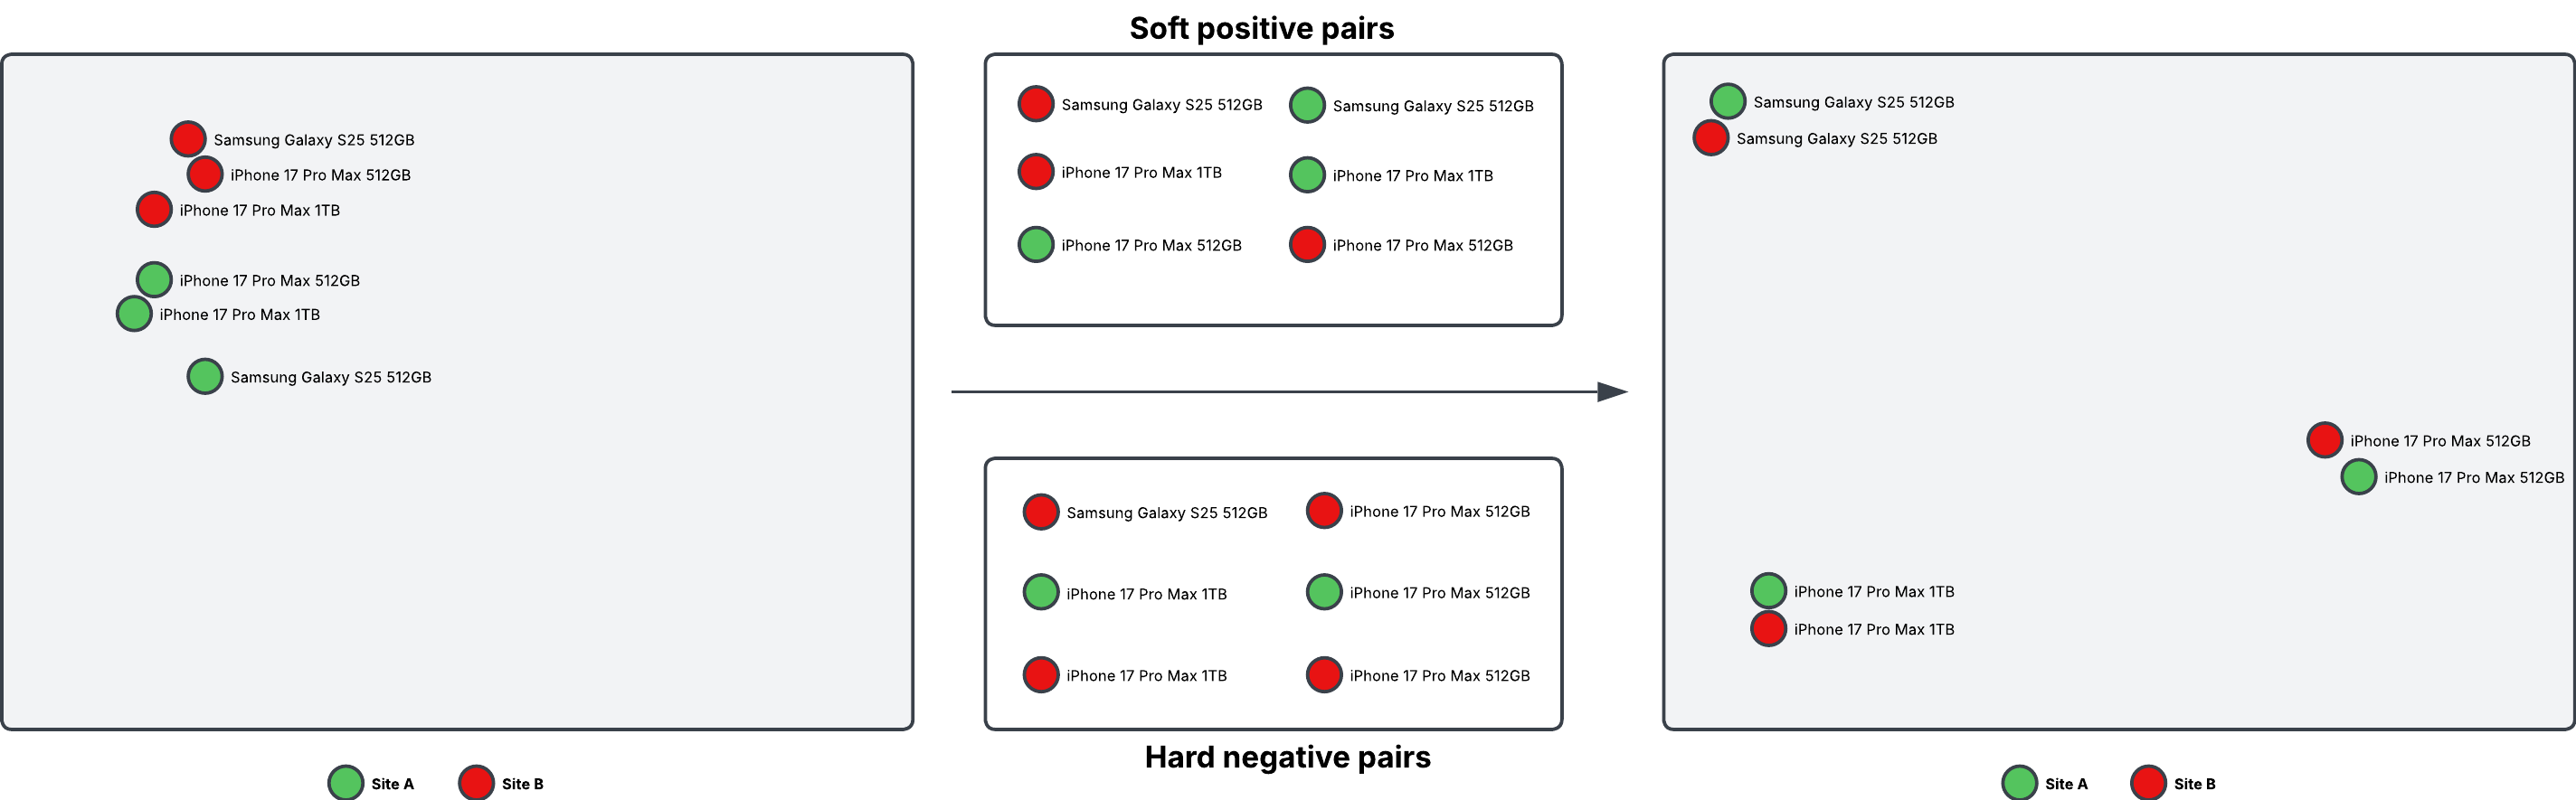
\includegraphics[width=1\textwidth]{images/contrastive_finetuning}
    \caption{How contrastive fine-tuning can bring similar products closer together in the embedding space, while pushing dissimilar products further apart.}
    \label{fig:contrastive_finetuning}
\end{figure}

Nearly 2000 product pairs were manually labelled as either matching or non-matching, and these were used to fine-tune the pre-trained RexBERT model on the body of each page's minimized content.
These pairs were selected to be a mix of both soft positive pairs and hard negative pairs, in order to provide the model with a diverse set of examples to learn from.
Using a similar process to the page classification and information extraction models, the fine-tuned model was trained on AWS SageMaker using hyperparameter tuning, which enabled automatic selection of the best hyperparameters.

Using this approach, the model was able to learn a more robust representation of the product pages that captures the semantic similarity between them, which improved the performance of the product matching module.
When using the embeddings generated by this fine-tuned model, the average similarity scores for matching and non-matching products were \texttt{0.896} and \texttt{0.356} respectively, with a difference of \texttt{0.540} and a percentage difference of \texttt{151.69\%} \footnote{These results differ from the results obtained in the final evaluation phase in section~\ref{sec:product_matching_evaluation} as the evaluation was performed using a larger training dataset}, which was a significant improvement over the original embeddings generated by the pre-trained model, which had a difference of only \texttt{0.06} and a percentage difference of \texttt{6.98\%}.
This shows that the fine-tuned model was able to learn a more discriminative representation of the product pages that captures the semantic similarity between them, which improved the performance of the product matching module.

\subsubsection{Vector Generation Phase}\label{subsubsec:sec_product_matching_vector_generation_phase}
In this phase, the fine-tuned model is used to generate vector representations for all product pages in the database.
This is done by passing the text content of the minimized HTML of each product page through the fine-tuned model to obtain the corresponding embedding vector.
These embedding vectors are then stored in the PostgreSQL database.
PostgreSQL allows for the storage of vector data types, using the \texttt{pgvector} extension, which allows for efficient storage, retrieval and comparison of vector data.
Figure~\ref{fig:vector_generation_phase} illustrates how the vector generation phase is used to generate vector representations for all product pages in the database.

\begin{figure}
    \centering
    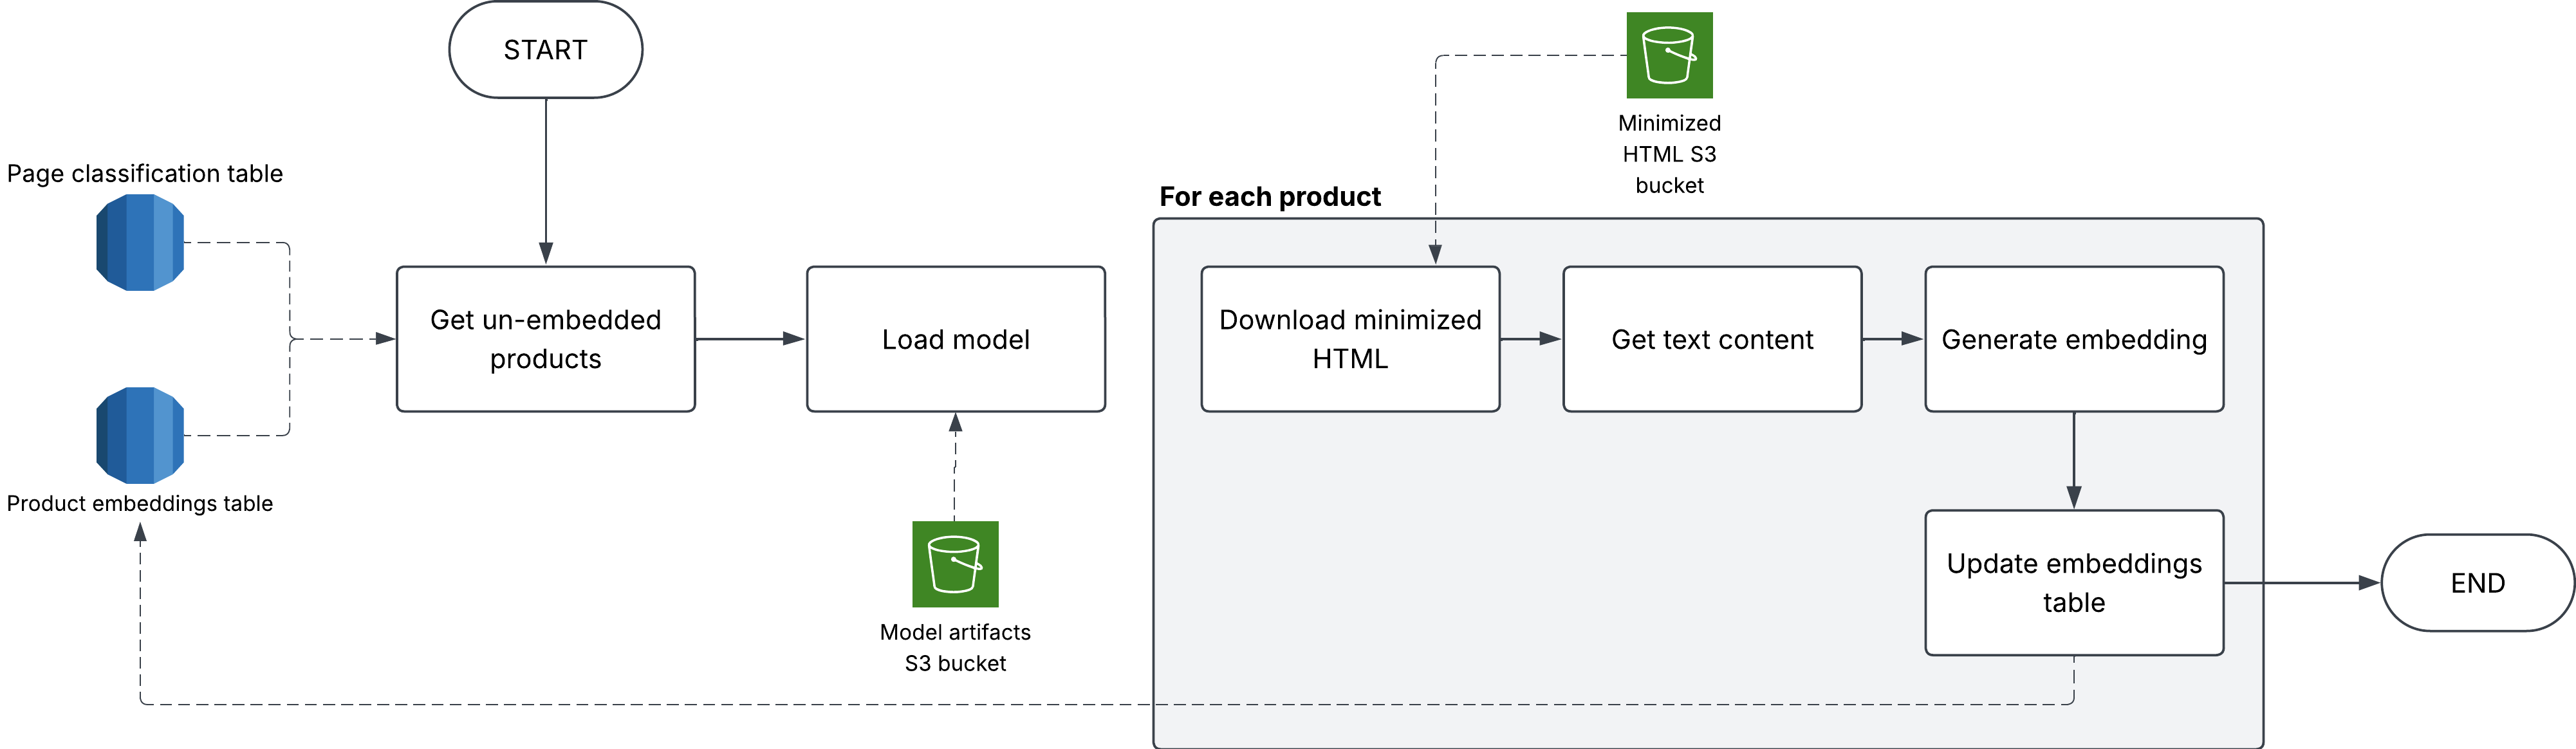
\includegraphics[width=1\textwidth]{images/generating_embeddings}
    \caption{Overview of the vector generation phase.}
    \label{fig:vector_generation_phase}
\end{figure}

Even though the vector generation phase is a computationally expensive process, it is only done once for each product page, and the resulting embeddings can be reused for all subsequent candidate pairs that involve that product page.
Therefore, the computational cost of this phase is spread out over all subsequent candidate pairs that involve that product page, which makes it a relatively efficient process in the long run.

\subsubsection{Matching Phase}\label{subsubsec:sec_product_matching_matching_phase}
In this phase, the vector representations of the candidate pairs are compared using cosine-similarity, and a threshold is set to determine whether the candidate pairs are considered to be matching or not.
This could be done entirely within the PostgreSQL database, using the \texttt{pgvector} extension to compute the cosine similarity between the embedding vectors of the candidate pairs, and then applying a threshold to determine whether the candidate pairs are considered to be matching or not.
Different values for this threshold were experimented with, and \texttt{0.691} was found to provide the highest F1 score.
However, this threshold was left to be configurable to be able to adjust it based on user preferences, as some users may prefer to have a higher precision at the cost of recall, while others may prefer to have a higher recall at the cost of precision.